\section{New Method}
In order to estimate the performance-per-watt of a multi-core chip for different number of 
active cores and various active core distributions, we first propose an iteration based 
full-chip power estimation method, which can apply the thermal model into the analysis of
performance-per-watt of multi-core chips. Furthermore, a non-iteration based method is 
proposed, which can implement local linearization to avoid time-consuming iterations. 
Additionally, a greedy based method can be integrated into the non-iteration based power
estimation method to achieve further acceleration.

\subsection{Iteration based leakage-aware power estimation}
Because of the dependency of static power on temperature, it's not straightforward to compute
the static power and temperature of next steady state based on current static power and 
temperature. Iteration method can be implemented to solve such problem, the computation flow 
is shown in Fig.x.

The initial value of $P^0_s(T,t+h)$ is a guess we provide based on the process technology.
The temperature distribution $T(t+h)^0$ can be calculated with such guess. $P^1_s(T,t+h)$,
the static power of next time step is updated with $T(t+h)^0$. Next, the temperature 
distribution $T(t+h)^1$ can be derived from $P^1_s(T,t+h)$, which concludes one iteration
loop. Such iteration goes on until the convergence test is satisfied as 
$\parallel P^i_s(T,t+h)$-$P^(i-1)_s(T,t+h)\parallel<\epsilon$. Finally, the static power and
temperature of steady state is outputted.

The iteration based method can produce an accurate outcome providing the $\epsilon$ is 
chosen to be small enough, yet the computing time is a serious problem, especially when the
number of cores is large enough.

\subsection{Local linearized thermal model}
The major difficulty of calculating leakage-aware power estimation comes from the nonlinear 
thermal model shown in (x), which is caused by the nonlinear relation between subthreshold 
current and temperature.

To reduce the long computing time caused by iteration method, the leakage current $I_{leak}$ 
can be linearized to eliminate the non-linearity between $p_{s}$ and temperature, thus 
accelerating the computation.
Taylor expansion is performed on the original $I_{leak}$ model at a expansion point $T_{0}$. 
Thus the linearized relation of $I_{leak}$ and temperature is obtained as:
\begin{equation}\label{linear_subthreshold}
\begin{split}
I_{sub} = &K(\frac{k}{q})^{2}e^(\frac{q(V_{GS}-V{th})}{\eta kT_{p0}}\\
&\times (T_{p0}^{2}+(2T_{p0}-\frac{q(V_{GS}-V_{th})}{\eta k})(T_{p}-T_{p0}))\\
&+ o[(T_{p}-T_{p0})^{2}].
\end{split}
\end{equation}

The relation between static power and temperature in linear form can also be achieved as:
\begin{equation}\label{linear_static}
\begin{split}
p_{s} &= V_{dd}I_{leak}\\
&= V_{dd} \times (I_{lin}+I_{gate})\\
&= V_{dd} \times (I_{lin}(T_{p})+I_{const})
\end{split}
\end{equation}

The linearized static power equation in matrix form is
\begin{equation}\label{linear_static_matrix}
P_{s} = P_{0}+A_{s}T
\end{equation}

\subsection{Non-iteration based power estimation}

\subsection{Greedy based acceleration of power estimation}
In previous sections, to find the optimal active core distribution which leads to highest 
performance-per-watt, for a $n$-core system with different active core numbers,  a 
combinational method with high complexity is implemented. However, it's  especially 
impractical when the number of cores is too big. Therefore, a greedy based method which can
find a sub-optimal active core distribution with much less time consumption is applied.




In the coming many-core era, due to the tight power budget, power efficiency is cricital for
many-core processor design. In the previous work by Dong Hyuk Woo, evaluation of energy
efficiency on the basis of performance and power (PPW) models is developed, which shows the
tendency of PPW with number of cores. We implement the dark silicon and thermal model into the
evaluation of PPW to gain a better understanding of PPW in the dark silicon era.

It is widely acknowledged that the total power of a chip is composed of dynamic and 
static power. The dynamic power is dependent on the activities of the chip, therefore it's 
easily estimated by methods such as performance counter.
Yet the static power $p_{s}$ of the chip is mainly affected by temperature, for it's caused by
leakage current $I_{leak}$ as
\begin{equation}\label{ps}
p_{s} = V_{dd}I_{leak}
\end{equation}

Due to the non-linear relationship between $I_{leak}$ and temperature, $p_{s}$ cannot be
calculated directly. The iteration method is traditionally implemented to solve such problems.







The average power consumption of the many-core processor is as follows:
\begin{equation}\label{average_power}
W = \frac{P_{1} \times (1-f)+P_{n} \times f/n}{(1-f)+f/n}
\end{equation}

$P_{1}$ is the power consumption during the sequential computation phase, $P_{n}$ is the power 
consumption during the parallel computation phase. 

$Perf/W$ of a many-core processor is expressed as

\begin{equation}\label{ppw}
\begin{split}
\frac{Perf}{W} &= \frac{1}{(1-f)+f/n} \times \frac{(1-f)+f/n}{P_{1} \times (1-f)+P_{n} \times f/n}\\
&= \frac{1}{P_{1} \times (1-f)+P_{n} \times f/n}
\end{split}
\end{equation}


\subsection{Power consumption with thermal constraints}
$P_{n}$ is made up of the power consumption of n active cores. Please note that in dark silicon
era, $P_{n} = nk$ is not the correct expression. Due to thermal constraint, Dynamic Voltage and
Frequency Scaling(DVFS) is necessary for Thermal Design Power(TDP) consideration. As a result,
the power consumption of each of the core may decrease with the increase of the number of active cores.
From xx, we have
\begin{equation}\label{gt=bp}
(G - B_{c}A_{s})T(t) + C\frac{dT(t)}{dt}= B_{c}(P_{d}(t) + P_{0})
\end{equation}

By applying thermal model, the effect of temperature on cores can be introduced. 
Through ergodic method, the distribution of light core with the maximum PPW
for number of light core from 1 to n can be specified.

In (2) and (3), $P_{1}$ is consisted of the power consumption of n-1 idle cores and 1 active 
core. The expression of $P_{1} = 1+(n-1)k$ is not implemented, for the power consumption of 
idle cores and active core is not consistant, due to the influence of the temperature.

By appending idle core model into the above mentioned thermal model, the distribution of idle
core and active core with the maximum PPW for number of light core from 1 to n can be specified.

\subsection{}

\begin{figure}
\centering
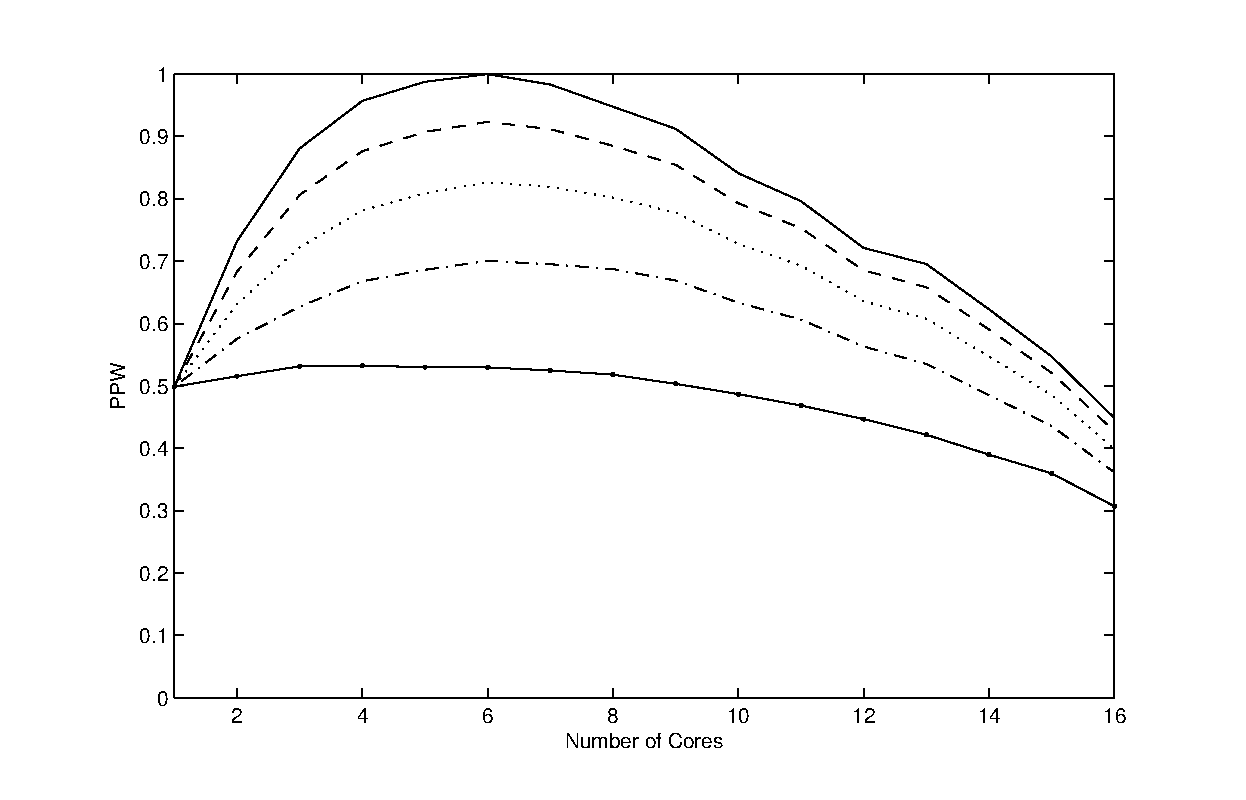
\includegraphics[width=1\columnwidth]{fig/ppw_alpha_ratio.eps}
\caption{The relation between PPW and the number of cores.
}
\label{fig:ppw_alpha_ratio}
\end{figure}